\documentclass[a4paper]{article}
%\usepackage[latin1s]{inputenc}
\usepackage{mypack}
\usepackage[ampersand]{easylist}
\usepackage{fullpage}
\setlength{\parindent}{0cm}
\begin{document}

\section{Usecases}
\begin{center}
	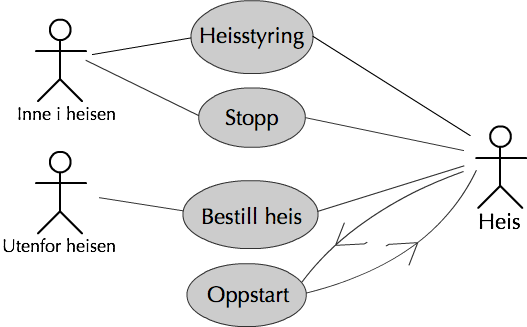
\includegraphics[width=0.7\textwidth]{grafikk/usecase.png}\\
\end{center}
\emph{
Bestillingsknapp: Knappene opp og ned som befinner seg i hver etasje.\\
Etasjeknapp: Knappene inne i heisen som bestemmer hvor heisen skal g�
}

%####################
\subsection*{Oppstart}
\begin{minipage}{0.47\textwidth}
\underline{Precondition:} 
Ingen

\underline{Trigger:}  
Program startes

\underline{Suksesscenario:}
\begin{enumerate}
	\item Sjekk etasjesensor
	\item Kj�r heis opp til den kommer til en etasje
	\item Stopp heisen
\end{enumerate}

\end{minipage}
\hfill
\begin{minipage}{0.47\textwidth}
\underline{Utvidelser:}

\begin{description}                                                                      
\item 1a. Hvis heis er i etasje, hopp til punkt 3.
\end{description}

\underline{Suksessgaranti:} 
Heis i ro i kjent etasje

\underline{Minimal garanti:} 
samme som suksessgaranti 

\end{minipage}


%#####################
\subsection*{Stopp}
\begin{minipage}{0.47\textwidth}
\underline{Precondition:} 
Ingen

\underline{Trigger:} 
Stopp-knapp trykkes eller obstruksjon aktiveres n�r heisen er i bevegelse mellom etasjer

\underline{Suksesscenario:}
\begin{enumerate}
	\item Heisen stoppes
	\item Alle bestillinger slettes fra bestillingsliste
	\item For � komme ut av stopp-modus m� obstruksjon v�re av og etasjeknapp m� trykkes
\end{enumerate}
\end{minipage}
\hfill
\begin{minipage}{0.47\textwidth}
\underline{Suksessgaranti:}
\begin{enumerate}
	\item Heisen st�r stille
	\item bestillingene slettes
\end{enumerate}

\underline{Minimal garanti:} 
Samme som suksessgaranti

\underline{Scenario:} 

\end{minipage}

%####################
\subsection*{Bestill Heis}
\begin{minipage}{0.47\textwidth}
\underline{Precondition:} 
Stoppknappen har ikke blitt trykket, heis ikke i oppstartsmodus

\underline{Trigger:} 
Bestillingsknapp trykkes inn

\underline{Suksesscenario:} 
\begin{enumerate}
	\item Bestilling i etasje blir lagt til i ordreliste
	\item Heisen fortsetter med andre ordre. En ordre vil slettes etter at den blir ekspedert
	\item Hvis heisen ikke har flere ordre videre i retningen den sist kj�rte, vil den snu og ekspedere ordre i motsatt retning.
	\item N�r heisen kommer til riktig etasje, stopp heisen
	\item Fjern etasjen fra ordrelisten, �pne d�ren
	\item D�ren vil holdes �pen s� lenge det er obstruksjon. 
	\item N�r obstruksjonen fjernes vil d�ren holdes �pen i 3 sekunder.
\end{enumerate}
\end{minipage}
\hfill
\begin{minipage}{0.47\textwidth}
\underline{Utvidelser:}
\begin{description}
	\item 2a. Hvis heisen kommer til riktig etasje i samme retning som bestillingen, hopp til punkt 4.
	\item 6a. Hvis det ikke er obstruksjon, hold d�ren oppe i 3 sekunder. 
\end{description}

\underline{Suksessgaranti:} 
\begin{enumerate}
	\item Heisen st�r i etasjen
	\item D�r �pen i minimum 3 sekunder, deretter lukkes den hvis det ikke er obstruksjon
	\item Heisen vil fortsette i samme retning som bestillingen antyder
\end{enumerate}

\underline{Minimal garanti:} 
\begin{enumerate}
	\item Ingen
\end{enumerate}
\end{minipage}

%####################
\subsection*{Bestilling fra etasjeknapp}
\begin{minipage}{0.47\textwidth}
\underline{Precondition:} 
Heis ikke i oppstartsmodus 

\underline{Trigger:} 
Etasjeknapp trykket

\underline{Suksesscenario:}
\begin{enumerate}
	\item Bestilling i etasje blir lagt til i ordreliste
	\item Heisen med samme retning som f�r, og stopper for � ekspedere ordre.
	\item Hvis heisen ikke har flere ordre videre i retningen den sist kj�rte, vil den snu og ekspedere ordre i motsatt retning.
	\item N�r heisen kommer til riktig etasje, stopp heisen
	\item Fjern etasjen fra ordrelisten, �pne d�ren
	\item D�ren vil holdes �pen s� lenge det er obstruksjon. 
	\item N�r obstruksjonen fjernes vil d�ren holdes �pen i 3 sekunder.
\end{enumerate}
\end{minipage}
\hfill
\begin{minipage}{0.47\textwidth}
\underline{Utvidelser:}
\begin{description}
\item 2a. Hvis heisen kommer til bestillt etasje, hopp til punkt 4.
\end{description}
\underline{Suksessgaranti:} 
\begin{enumerate}
	\item Heis til etasje
	\item D�r �pen i minimum 3 sekunder, deretter lukkes den hvis det ikke er obstruksjon
\end{enumerate}

\underline{Minimal garanti:} 
Samme som suksessgaranti
\end{minipage}



%END USE_CASE
\section{Systemarkitektur}
\begin{figure}
\label{fig:sysArk}
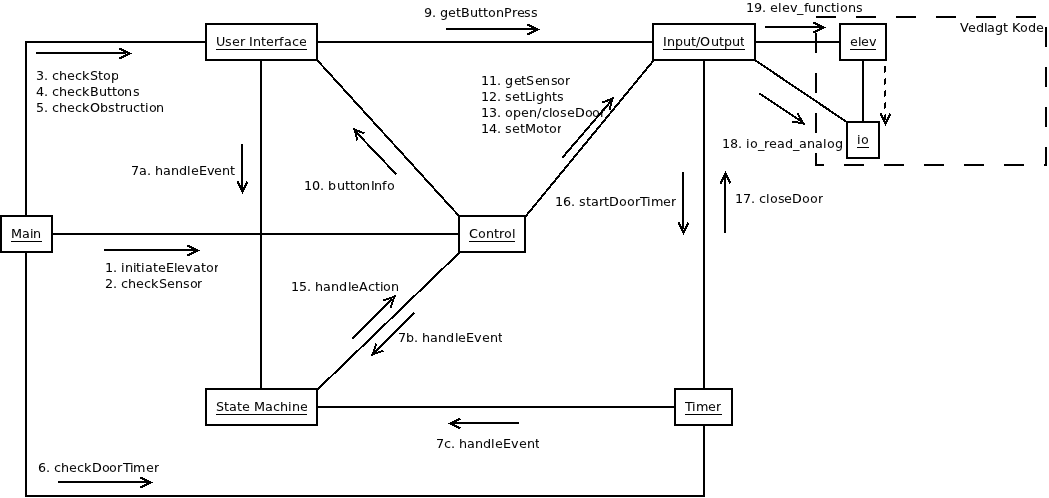
\includegraphics[width=\textwidth]{grafikk/systemarkitektur.png}
\caption{Overordnet systemarkitektur}
\end{figure}
\begin{description}
\item[1.] initiateElevator kalles hver gang heisprogrammet starter, og utf�rer oppstartsprosedyren beskrevet i Usecase-diagrammet.
\item[2. - 6.] check-funksjonene kalles kontinuerlig i main, og registrerer hendelser for tilstandsmaskinen.
\item[7.] handleEvent kalles av check-funksjonene i tre forskjellige klasser. HandleEvent kalles med et av argumentene NEW\_DESTINATION, FLOOR\_REACHED, STOP\_PRESSED og ORDER\_BUTTON\_PRESSED avhengig av hvilke hendelser check-funksjonene registrerer.
\item[8.] handleAction er et samlebegrep for handle-funksjonene som kalles av tilstandsmaskinen. 
\item[9.] betingelser er funksjoner som returnerer 0 eller 1. Disse m� v�re oppfylt (returnerer 1) for � f� en transisjon i tilstandsmaskinen der disse er satt som betingelse.
\item[10.] getUiSignals er et samlebegrep for funksjonene som henter signaler fra knappene og obstruksjon. Funksjonene kalles av check-funksjonene.
\item[11.] Siste bestillingsknapp som trykkes, lagres i ui-klassen, og getLastOrder returnerer denne til kontroll-klassen. 
\item[12.] getSensor er et samlebegrep for funksjoner som henter informasjon fra etasjesensorene. 
\item[13.] controlLights er et samlebegrep for funksjoner som skrur av og p� lys.
\item[14.] openDoor og closeDoor h�ndterer d�ra.
\item[15.] controlMotor er et samlebegrep for funksjoner som starter og stopper motoren.
\item[16.] startDoorTimer kalles n�r d�ra �pnes for � telle ned tre sekunder.
\item[17.] closeDoor kalles fra timer-klassen og lukker d�ra n�r timeren har telt ned.
\item[18.] io\_read\_analog er en funksjon som returnerer m�lt motorhastighet.
\item[19.] elevFunctions er funksjonene i det ferdige grensesnittet mot heisen.
\end{description}
\section{Klassediagrammer}
Heisstyringa er delt opp i klasser. M�ten vi har implementert dette p� er at alle variabler er deklarert static for � holde de internt i en klasse/fil, og innf�re set- og getfunksjoner der det trengs. Grunnen til denne oppdelingen er selvf�lgelig � f� en logisk oppdeling, hvor hver klasse har et veldefinert ansvarsomr�de. For hver klasse b�r det g� greit fram hva de forskjellige variablene og funksjonene gj�r, men det er gitt utdypende forklaring ved de mest sentrale.
\subsection{Tilstandsmaskinen}
\begin{figure}
\centering
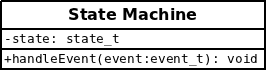
\includegraphics[scale=0.6]{grafikk/stateMachine.png}
\label{klasse:SM}
\caption{Klassediagram for tilstandsmaskinen}
\end{figure}
Tilstandsmaskinen holder orden p� hvilken tilstand heisen st�r i. 
\begin{description}
\item[handleEvent]\hfill \\
Bestemmer, sammen med tilstandsvariablen, nestetilstand og handling for heisen n�r den genererer en hendelse.
\end{description}
\subsection{Kontroll}
\begin{figure}
\centering
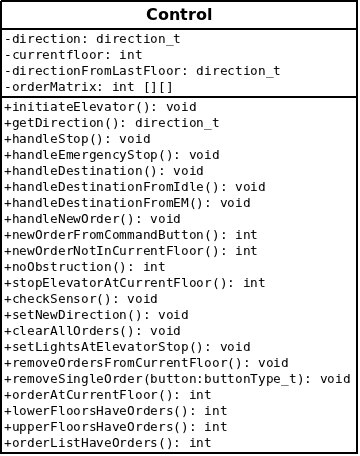
\includegraphics[scale=0.6]{grafikk/control.png}
\label{klasse:kontroll}
\caption{Klassediagram for kontrollklassen}
\end{figure}
Kontrollklassen inneholder alle funksjoner og variabler som h�ndterer logikken og den fysiske funksjonen i heisen, som � bestemme retning, at motoren skal startes, hvilke lys som skal tennes, holde orden p� bestillingene, og lignende.
\begin{description}
\item[Handlinger]\hfill \\
De forskjellige handlingene (handle$\cdots$) kalles av tilstandsmaskinen, og beskriver den overordnene oppf�rselen til heisen. Grunnen til tre forskjellige handleDestination-funksjoner er at man i n�dstopp- og idletilstand trenger litt annerledes rutiner for � bestemme neste m�l for heisen.
\item[Sperre? Vakt?]\hfill \\
newOrderFromCommandButton, newOrderNotInCurrentFloor, noObstruction og stopElevatorAtCurrentFloor er ?sperrer? tilstandsmaskinen bruker for � avgj�re om den skal utf�re handlingene.
\item[Checksensor]\hfill \\
En lyttefunksjon som st�r og g�r i main-funksjonen for � avgj�re hvilken etasje heisen er i, og gi en handling n�r den ankommer en etasje.
\item[Heisstyring]\hfill \\
setNewDirection, clearAllOrders, setLightsAtElevatorStop, removeOrdersFromCurrentFloor og removeSingleOrder er funksjoner som p�virker retning, ordre og lys for heisen.
\item[Sammeligning]\hfill \\ 
De fire nederste funksjonene er hjelpefunksjoner som bestemmes av ordrene heisen har. Brukes for � bedre lesbarhet og for � unng� for mye n�sting.
\end{description}
\subsection{User Interface}
\begin{figure}
\centering
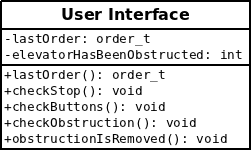
\includegraphics[scale=0.6]{grafikk/ui.png}
\label{klasse:ui}
\caption{Klassediagram for UI-klassen}
\end{figure}
Denne klassen s�rger for � h�ndtere input fra brukeren, som bestillingsknapper, stoppknapp og obstruksjonsf�leren i d�ra. Den s�rger for � sende bestillinger til kontroll.
\begin{description}
\item[Sjekkfunksjoner]\hfill \\
checkButtons, checkStop og checkObstruction l�per i main-funksjonen for � for � h�ndtere input fra brukeren. De genererer ogs� hendelser for tilstandsmaskinen.
\item[LastOrder]\hfill \\
Denne kalles av kontroll-klassen for � returnere siste ordreknapp som ble trykket inn og legge bestilling i ordrelisten.
\end{description}
\subsection{Timer}
\begin{figure}
\centering
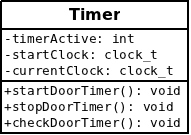
\includegraphics[scale=0.6]{grafikk/timer.png}
\label{klasse:timer}
\caption{Klassediagram for timeren}
\end{figure}
Timeren er en enkel klasse for � telle ned tre sekunder hver gang d�ren �pnes i en etasje. Den har to variabler fra time-biblioteket for � telle opp til 3 sekunder, og et heltall som holder orden p� om den er aktiv eller iikke.
\begin{description}
\item[checkDoorTimer]\hfill \\
Denne st�r ogs� og l�per i main-funksjonen, og sjekker om nedtellingen er ferdig eller ikke.
\end{description}
\subsection{I/O}
\begin{figure}
\centering
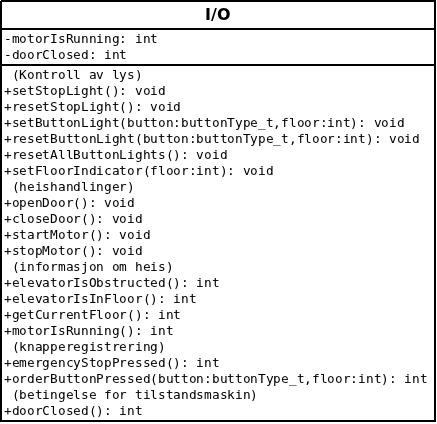
\includegraphics[scale=0.6]{grafikk/io.png}
\label{fig:class_ui}
\caption{Klassediagram for I/O-klassen}
\end{figure}
I/O klassen er en egenlagt driver for � styre heisen. Dette er v�r mest maskinn�re klasse, som inneholder funksjoner for alle hardware-relaterte operasjoner som � skru av og p� lys, gi signal fra sensoren og sette motorhastigheten. Disse funksjonene implementeres ved hjelp av medf�lgende funksjoner i elev.c og io.c
\begin{description}
\item[Lysfunksjoner]\hfill \\
Det er funksjoner for � skru lys av og p�. Bestillingslampene kan skrus av en og en, eller alle p� en gang som for en n�dstopp. Etasjelyset har ingen resetfunksjon, da kun et skal tennes av gangen, og derfor kan det ordnes i setfunksjonen.
\item[Heisaksjoner]\hfill \\
Funksjoner for d�r- og motorstyring. Det er egen motorstopp for n�dsituasjoner, {\Huge hvorfor?}
\item[Informasjon om Heis]\hfill \\
Funksjoner som registrerer fysisk informasjon om heisen
\item[Knapperegistreringer]
orderButtonPressed blir kalt fra kontroll hver gang man trykker en knapp, og legger etasje og knappetype inn i diagrammet.
\item[vakt? sikring?]\hfill \\
doorClosed er vakt? sikring? som brukes av tilstandsmaskinen.
\end{description}



\end{document}
